%% \documentclass[handout]{beamer}
\documentclass{beamer}
%% \usetheme{Copenhagen}
\usetheme[progressbar=foot]{metropolis}

%% \setbeameroption{show only notes}
 
\usepackage[utf8]{inputenc}
\usepackage{minted}
\usepackage{ulem}
\usepackage{appendixnumberbeamer}
\usepackage{fancyvrb}
\usepackage{tikz}
\usetikzlibrary{arrows.meta,positioning,hobby,calc}

  \tikzset{
    invisible/.style={opacity=0},
    visible on/.style={alt={#1{}{invisible}}},
    alt/.code args={<#1>#2#3}{%
      \alt<#1>{\pgfkeysalso{#2}}{\pgfkeysalso{#3}} % \pgfkeysalso doesn't change the path
    },
  }
 
\title{Formal(ish) NP-Hardness Proofs}
\subtitle{Or, How to Take a Long Time Proving Basic Things}
\author{John Grosen}
\date{8 May 2019}

%% \beamertemplatenavigationsymbolsempty

\begin{document}

\begin{frame}
  \titlepage

  \note[item]{I'm John Grosen, and I'm presenting my project on formal...ish NP-hardness proofs, or, how to take a long time proving basic things.}
  \note[item]{Well, you all already know what NP-hard means, so...}
\end{frame}

\section{Introduction}

\begin{frame}
  \frametitle{What is a formal proof?}
  \framesubtitle{(Haven't we been writing these all semester?)}

  \note[item]{...what \emph{is} a formal proof?}
  \note[item]{In this class, we've been using ``informal'' vs ``formal'' proofs to mean ``posts on Coauthor'' vs ``something for a journal''}
  \note[item]{However, for the sake of this talk it means something else: formal proofs are checkable by a computer.}

  Salient property for us:
  a formal proof is \emph{computer-checkable}.
\end{frame}

\begin{frame}
  \frametitle{Why do we want formal hardness proofs?}

  \vspace{-2ex}

  \begin{figure}
    \includegraphics[width=0.8\textwidth]{bug1header}
    $$\vdots$$
    \includegraphics[width=\textwidth]{bug1}
    $$\vdots$$
    \includegraphics[width=0.8\textwidth]{bug1footer}
  \end{figure}

  \centering
  Humans get things wrong!

  \note[item]{But why would care about whether a proof can be checked by a computer?}
  \note[item]{Well, humans aren't perfect!}
  \note[item]{And while computers aren't creative enough to derive interesting proofs, they are systematic enough to check them.}
\end{frame}

\begin{frame}
  \frametitle{Why do we want formal hardness proofs?}

  Formal proofs aren't a silver bullet: you still have to understand \emph{what}
  they're proving, which can be hard!

  \vspace{5ex}

  But this is often a worthy tradeoff.

  \note[item]{Of course, it isn't a perfect solution to the problem -- you have to know what the computer is checking.}
  \note[item]{But in lots of domains, that's a tradeoff that makes sense.}
  \note[item]{I think it particularly makes sense for reductions, where you typically have short specifications of what your problems are, but the proofs can be long and complex.}
  \note[item]{(pause)}
\end{frame}

\begin{frame}
  \frametitle{What is Coq?}

  \begin{figure}
    \includegraphics[height=0.4\textheight]{coq}
  \end{figure}

  Coq is
  \begin{itemize}
  \item an interactive theorem prover,
  \item based on functional programming,
  \item with a really fancy type system.
  \end{itemize}

  \note[item]{For this project, I used the theorem prover Coq, which is what Adam Chlipala's group here in CSAIL uses.}
  \note[item]{Coq is an interactive theorem prover based on functional programming combined with a powerful type theory.}
  \note[item]{You write code, which you can prove theorems about, which are themselves just code.}
  \note[item]{Anyway, how should we do hardness proofs in Coq?}
\end{frame}

\section{Hardness Proofs in Coq}

\begin{frame}
  \frametitle{How do we define NP-hardness in Coq?}

  Formally, perhaps we should define NP-hardness starting from nondeterministic Turing machines...

  %% \pause
  \vspace{5ex}

  ...but that sounds difficult, so let's just use Karp reductions starting from a well-known NP-hard problem: FORMULA-SAT.

  \note[item]{Perhaps we'd ideally like to start all the way up at defining nondeterministic Turing machines, and all that jazz.}
  \note[item]{...but that sounds like a lot of work for a class project, so instead I just fixed FORMULA-SAT as the ultimate NP-hard problem, and used Karp reductions down from there.}
\end{frame}

\begin{frame}
  \frametitle{What is a Karp reduction?}
  \framesubtitle{And how do we prove one valid?}

  \onslide<2->{To prove} a Karp reduction $A \leq B$ is valid\only<1>{ if it is}\only<2->{, we must}
  \vspace{3ex}

  \renewcommand{\arraystretch}{1.5}
  \begin{tabular}{rcc}
    & \onslide<3->{PL community?} & \onslide<5->{hardness community?} \\
    \textbf<7>{\onslide<2->{Prove} \onslide<1->{correct}\onslide<2->{ness}} & \textbf<7>{\action<3-|alert@3>{easy}} & \textbf<7>{\action<5-|alert@5>{hard}} \\
    \onslide<2->{Prove} \onslide<1->{polytime}\onslide<2->{ness} & \action<3-|alert@4>{hard} & \action<5-|alert@6>{easy} \\
  \end{tabular}
  \renewcommand{\arraystretch}{1}

  \note[item]{So, a Karp reduction requires two conditions for validity: correctness and polytimeness.}
  \note[item]{If you ask the programming languages community, they'll say proving correctness is easy, but polytimeness sounds tricky.}
  \note[item]{On the other hand, if you ask the hardness community, they'll say correctness is the challenging part, but polytimeness is trivial.}
  \note[item]{Given that my background is in PL, and I'm in a hardness class, you can probably guess which of these conditions I decided to focus on.}
\end{frame}

\begin{frame}[fragile]
  \frametitle{Encoding reductions in Coq}

  \begin{minted}{coq}
Class problem A :=
  { ProblemYes : A -> Prop;
  }.
  \end{minted}

  %% \pause

  \begin{minted}{coq}
Class reduction `(PA : problem A)
                `(PB : problem B)
                 (f : A -> B) :=
  { ReductionCorrect : forall x,
        ProblemYes x <-> ProblemYes (f x);
  }.
  \end{minted}

  \note[item]{So how do we encode reductions in Coq?}
  \note[item]{Well, we define a problem as a definition of whether an instance is a YES-instance or a NO-instance.}
  \note[item]{From there, a reduction is just a function $f$ from problem A to problem B, such that $x$ is a YES-instance of A if and only if $f(x)$ is a YES-instance of B.}
\end{frame}

\begin{frame}
  \frametitle{The state of our reductions}

  \centering
  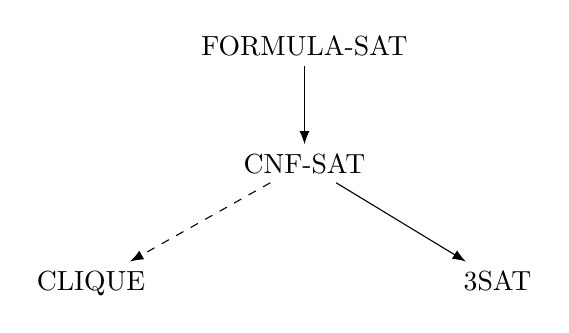
\begin{tikzpicture}
    \node (fs) {FORMULA-SAT};

    %% \pause
    \node[below=of fs] (cs) {CNF-SAT};
    \draw[-Latex] (fs) -- (cs);

    %% \pause
    \node[below right=of cs] (ts) {3SAT};
    \draw[-Latex] (cs) -- (ts);

    %% \pause
    \node[below left=of cs] (cl) {CLIQUE};
    \draw[-Latex, dashed] (cs) -- (cl);

    %% \pause
    %% \draw[red, thick, rotate=60, visible on=<5->] ($(cs)!0.5!(ts)$) ellipse[x radius=1,y radius=2.8];
  \end{tikzpicture}

  \note[item]{What reductions have we managed to prove?}
  \note[item]{Starting from FORMULA-SAT, I proved the reduction to CNF-SAT, and then to 3SAT.}
  \note[item]{I'm currently working on a reduction to CLIQUE.}
\end{frame}

\section{CNF-SAT $\leq$ 3SAT}

\note[item]{As a case study, let's look the reduction from CNF-SAT to 3SAT.}

\begin{frame}[fragile]
  \frametitle{CNF-SAT syntax}

  \begin{minted}[fontsize=\footnotesize]{coq}
Inductive literal :=
| PosLit : var -> literal
| NegLit : var -> literal
.
\end{minted}

  %% \pause
  \begin{minted}[fontsize=\footnotesize]{coq}
Definition clause : Type := list literal.
Definition cnf_formula : Type := list clause.
  \end{minted}

  \note[item]{We start out by defining the syntax for CNF-SAT:}
  \note[item]{A literal is either positive or negative, and both have a variable.}}
  \note[item]{A clause is just a list of literals, and a formula is just a list of clauses.}
\end{frame}


\begin{frame}[fragile]
  \frametitle{3SAT definition}

  \begin{minted}[fontsize=\footnotesize]{coq}
Definition threecnf_formula :=
  { f : cnf_formula | Forall (fun clause => length clause <= 3) f}.
  \end{minted}

  \note[item]{Then, a 3-CNF formula is just a CNF formula where all clauses have length less than or equal to 3.}
\end{frame}

\begin{frame}
  \frametitle{Karp's ``Proof''}

  \includegraphics[width=\textwidth]{karp_3sat}

  $\ldots$

  \includegraphics[width=\textwidth]{karp_excerpt}

  \note[item]{Now, if we look at Karp's proof of this reduction, you'll notice that there's not much of a proof here beyond the reduction itself.}
  \note[item]{Indeed, Karp rather explicitly leaves the proof as an exercise to the reader.}
  \note[item]{So we're largely on our own.}
\end{frame}

\begin{frame}
  \frametitle{Clause reduction example}

  $$ (l_1 \lor l_2 \lor l_3 \lor l_4 \lor l_5) $$
  \par
  $$\Rightarrow$$
  \pause
  $$ (l_1 \lor l_2 \lor c_1) \land (\bar{c_1} \lor l_3 \lor c_2) \land (\bar{c_2} \lor l_4 \lor l_5) $$

  \note[item]{Let's first look at an example of the reduction for a single clause.}
  \note[item]{The idea is that we add more free variables in order to give the choice of satisfying any of the five literals, even through they're split up across three conjoined clauses.}
  \note[item]{Here $c_1$ and $c_2$ are what I call the carry variables.}
\end{frame}

\begin{frame}[fragile]
  \frametitle{Clause reduction with carry}

  \begin{minted}[fontsize=\footnotesize]{coq}
Fixpoint clause_to_three_carry (cl : clause)
                               (carry : var) : Fresh (list clause) :=
  match cl with
  | []
  | [_] =>
    ret [] (* error case *)
  | [a; b] =>
    ret [ [NegLit carry; a; b] ]
  | a :: cl' =>
    x <- fresh ;;
    rest <- clause_to_three_carry cl' x ;;
    ret ([NegLit carry; a; PosLit x] :: rest)
  end.
  \end{minted}

  \note[item]{Here's the actual code the implements the meat of the reduction.}
\end{frame}

\begin{frame}[fragile]
  \frametitle{\texttt{clause\_to\_three\_carry} correctness}

  \only<1>{\inputminted[fontsize=\scriptsize]{coq}{clause_to_three_carry.v}}
  \only<2>{\inputminted[fontsize=\scriptsize, highlightlines={5}]{coq}{clause_to_three_carry.v}}
  \only<3>{\inputminted[fontsize=\scriptsize, highlightlines={6-10}]{coq}{clause_to_three_carry.v}}
  \only<4>{\inputminted[fontsize=\scriptsize, highlightlines={11-15}]{coq}{clause_to_three_carry.v}}
  \only<5>{\inputminted[fontsize=\scriptsize, highlightlines={16-19}]{coq}{clause_to_three_carry.v}}
  %% \begin{minted}[fontsize=\footnotesize]{coq}
  %% \end{minted}
\end{frame}

\begin{frame}[fragile]
  \frametitle{...and eventually, NP-hardness}

  \begin{minted}[fontsize=\footnotesize]{coq}
Theorem three_sat_is_np_hard : np_hard ThreeSAT.
Proof.
  apply (np_hard_reduction CNFSAT) with (f := cnf_to_three).
  { apply cnf_sat_is_np_hard. }
  { auto using cnf_to_three_correct. }
Qed.
  \end{minted}
\end{frame}

\section{Conclusion}

\begin{frame}
  \frametitle{Moral of the story?}

  Doing formal proofs of reductions, even simple ones like Karp's, is quite a
  pain. But you really get to understand the proofs.
\end{frame}

\begin{frame}
  \frametitle{Future work}

  It would be cool to do all of Karp's reductions!

  Ideally we'd also prove polytimeness somehow.
\end{frame}

\appendix{Backup slides}

\begin{frame}[fragile]
  \frametitle{CNF-SAT semantics}

  \begin{minted}[fontsize=\footnotesize]{coq}
Definition satisfies_literal (a : assignment)
                             (l : literal) : bool :=
  match l with
  | PosLit v => a v
  | NegLit v => negb (a v)
  end.
  \end{minted}

  \pause
  \begin{minted}[fontsize=\footnotesize]{coq}
Fixpoint satisfies_clause (a : assignment)
                          (c : clause) : bool :=
  match c with
  | nil => false
  | l :: c' => satisfies_literal a l || satisfies_clause a c'
  end.
  \end{minted}
\end{frame}

\begin{frame}[fragile]
  \frametitle{CNF-SAT semantics}

  \begin{minted}[fontsize=\footnotesize]{coq}
Fixpoint satisfies_cnf_formula (a : assignment)
                               (f : cnf_formula) : bool :=
  match f with
  | nil => true
  | c :: f' => satisfies_clause a c && satisfies_cnf_formula a f'
  end.
  \end{minted}

  \pause
  \begin{minted}[fontsize=\footnotesize]{coq}
Definition cnf_satisfiable (f : cnf_formula) : Prop :=
  exists (a : assignment), satisfies_cnf_formula a f = true.
  \end{minted}
\end{frame}

\begin{frame}[fragile]
  \frametitle{Fresh}

  \begin{minted}[fontsize=\footnotesize]{coq}
Definition Fresh A :=
  N -> N * A.

Instance Monad_Fresh : Monad Fresh :=
  {| ret := fun _ x n => (n, x);
     bind := fun _ _ c1 c2 n => let (n', x) := c1 n in
                             c2 x n';
  |}.

Definition fresh : Fresh N :=
  fun n => (n + 1, n)%N.
  \end{minted}
\end{frame}

\begin{frame}[fragile]
  \frametitle{Single-clause reduction}

  \begin{minted}[fontsize=\footnotesize]{coq}
Definition clause_to_three (cl : clause) : Fresh (list clause) :=
  match cl with
  | []
  | [_]
  | [_; _]
  | [_; _; _] =>
    ret [ cl ]
  | a :: b :: cl' =>
    x1 <- fresh ;;
    many <- clause_to_three_carry cl' x1 ;;
    ret ([a; b; PosLit x1] :: many)
  end.
  \end{minted}
\end{frame}

\appendix{A Brief Tour of Coq}

\begin{frame}
  \frametitle{How do you use Coq?}

  As an example, let's prove the closed form of triangular numbers:
  $$ \forall n \geq 0, \,\, \sum_{i = 0}^n i = \frac{n (n + 1)}{2} $$
\end{frame}

\begin{frame}[fragile]
  \frametitle{How do you use Coq?}
  \framesubtitle{Theorem statement}

  \begin{minted}{coq}
Fixpoint sum_from_0_to (n : nat) : nat :=
  match n with
  | 0 => 0
  | S n' => n + sum_from_0_to n'
  end.
  \end{minted}

  \pause

  \begin{minted}{coq}
Lemma sum_from_0_to_spec : forall n,
    2 * sum_from_0_to n = n * (n + 1).
  \end{minted}
\end{frame}

\begin{frame}[fragile]
  \frametitle{How do you use Coq?}
  \framesubtitle{Proof}

  %% \addtolength{\tabcolsep}{-10pt}

  \begin{columns}

    \begin{column}{0.35\textwidth}

    \minipage[c][0.65\textheight][s]{\columnwidth}
    \footnotesize
    \begin{semiverbatim}
Proof.\onslide<2->
  induction n.\onslide<3->
  -\onslide<4-> simpl.\onslide<5->
    reflexivity.\onslide<6->
  -\onslide<7-> simpl.\onslide<8->
    rewrite mul_succ_r.\onslide<9->
    rewrite <-IHn.\onslide<10->
    omega.\onslide<11->
Qed.
    \end{semiverbatim}
    \endminipage
    \end{column}

    \begin{column}{0.7\textwidth}
    \footnotesize
    \onslide<1->
    \begin{onlyenv}<1>
    \minipage[c][0.65\textheight][s]{\columnwidth}
    \begin{minted}{coq}
1 subgoal (ID 4)
  
============================
forall n : nat,
  2 * sum_from_0_to n = n * (n + 1)
    \end{minted}
    \endminipage
    \end{onlyenv}

    \begin{onlyenv}<2>
    \minipage[c][0.65\textheight][s]{\columnwidth}
    \begin{minted}{coq}
2 subgoals (ID 9)
  
============================
  2 * sum_from_0_to 0 = 0 * (0 + 1)

subgoal 2 (ID 12) is:
 2 * sum_from_0_to (S n) = S n * (S n + 1)
    \end{minted}
    \endminipage
    \end{onlyenv}

    \begin{onlyenv}<3>
    \minipage[c][0.65\textheight][s]{\columnwidth}
    \begin{minted}{coq}
1 subgoal (ID 9)
  
  ============================
  2 * sum_from_0_to 0 = 0 * (0 + 1)
    \end{minted}
    \endminipage
    \end{onlyenv}

    \begin{onlyenv}<4>
    \minipage[c][0.65\textheight][s]{\columnwidth}
    \begin{minted}{coq}
1 subgoal (ID 21)
  
  ============================
  0 = 0
    \end{minted}
    \endminipage
    \end{onlyenv}

    \begin{onlyenv}<5>
    \minipage[c][0.65\textheight][s]{\columnwidth}
    \begin{minted}{coq}
1 subgoal (ID 12)

subgoal 1 (ID 12) is:
 2 * sum_from_0_to (S n) = S n * (S n + 1)
    \end{minted}

    \vspace{5ex}

    \textit{This subproof is complete,}\\
    \hspace*{2em}\textit{but there are some unfocused goals.}

    \textit{Focus next goal with bullet -.}
    \endminipage
    \end{onlyenv}

    \begin{onlyenv}<6>
    \minipage[c][0.65\textheight][s]{\columnwidth}
    \begin{minted}{coq}
1 subgoal (ID 12)
  
  n : nat
  IHn : 2 * sum_from_0_to n = n * (n + 1)
  ============================
  2 * sum_from_0_to (S n) = S n * (S n + 1)
    \end{minted}
    \endminipage
    \end{onlyenv}

    \begin{onlyenv}<7>
    \minipage[c][0.65\textheight][s]{\columnwidth}
    \begin{minted}{coq}
1 subgoal (ID 36)
  
  n : nat
  IHn : 2 * sum_from_0_to n = n * (n + 1)
  ============================
  S (n + sum_from_0_to n +
     S (n + sum_from_0_to n + 0)) =
  S (n + 1 + n * S (n + 1))
    \end{minted}
    \endminipage
    \end{onlyenv}

    \begin{onlyenv}<8>
    \minipage[c][0.65\textheight][s]{\columnwidth}
    \begin{minted}{coq}
1 subgoal (ID 37)
  
  n : nat
  IHn : 2 * sum_from_0_to n = n * (n + 1)
  ============================
  S (n + sum_from_0_to n +
     S (n + sum_from_0_to n + 0)) =
  S (n + 1 + (n * (n + 1) + n))
    \end{minted}
    \endminipage
    \end{onlyenv}

    \begin{onlyenv}<9>
    \minipage[c][0.65\textheight][s]{\columnwidth}
    \begin{minted}{coq}
1 subgoal (ID 38)
  
  n : nat
  IHn : 2 * sum_from_0_to n = n * (n + 1)
  ============================
  S (n + sum_from_0_to n +
     S (n + sum_from_0_to n + 0)) =
  S (n + 1 + (2 * sum_from_0_to n + n))
    \end{minted}
    \endminipage
    \end{onlyenv}

    \begin{onlyenv}<10>
    \minipage[c][0.65\textheight][s]{\columnwidth}
    \vspace{40ex}

    \textit{No more subgoals.}
    \endminipage
    \end{onlyenv}

    \begin{onlyenv}<11>
    \minipage[c][0.65\textheight][s]{\columnwidth}
    \vspace{40ex}

    \textit{sum\_from\_0\_to\_spec is defined}
    \endminipage
    \end{onlyenv}

    \end{column}
  \end{columns}
\end{frame}

\begin{frame}
  \centering
  \includegraphics[height=0.7\textheight]{pythagoras}
  \par
  \vspace{4ex}
  Pythagoras would be proud.
\end{frame}

\end{document}
